\chapter{Filtro de Kalman \textit{Unscented}}
\label{chapter:unscented}

Finalizada nossa discussão sobre o Filtro de Correntropia, seguiremos agora para o último método a ser explorado no projeto. O Filtro de Kalman \textit{Unscented}, apresentado originalmente em~\cite{julier-1997}, surgiu como uma alternativa ao Filtro de Kalman Estendido~\cite{sorenson-1985}; a proposta de ambos é generalizar o Filtro de Kalman~\cite{hayes-1996} para sistemas não-lineares. O modelo se baseia na transformação \textit{unscented}, a qual gera um conjunto estratégico de pontos associados 
à variável aleatória para estimar efetivamente a média e covariância de seu mapeamento não-linear. Ao contrário dos outros algoritmos do trabalho, a filtragem é em tempo real, ou seja, apenas amostras passadas (e presentes) são usadas no processo de estimação, embora possamos utilizar informações globais dos sinais nas condições iniciais.

A seção a seguir formula o problema, que é descrito na forma de uma representação em espaço de estados. Então, a intuição (com as equações) por trás do Filtro de Kalman será brevemente discutida. Em seguida, apresentaremos a transformação \textit{unscented}, para que o algoritmo do Filtro de Kalman \textit{Unscented} possa ser especificado. Finalmente, o modelo específico estruturado para o projeto será definido, e os resultados dos experimentos executados serão comentados.

\section{Formulação do problema}
\label{section:unscented:formulation}

Todos os estimadores discutidos até agora objetivaram computar, a partir de um sinal de entrada e uma observação, apenas a saída do sistema de interesse. Os filtros que discutiremos agora se diferenciam dos outros métodos por estimarem também os \emph{estados} do modelo. Precisamos então formular o novo problema em questão.

Na literatura, é possível encontrar diferentes formulações associadas ao algoritmo; muitas vezes, não há sinal de entrada no sistema, ou os ruídos são considerados não-aditivos. A discussão do capítulo será quase que inteiramente baseada no modelo apresentado no artigo original do Filtro de Kalman \textit{Unscented}~\cite{julier-1997}, já que suas hipóteses são suficientes para o contexto do trabalho. Considere então o sistema não-linear discreto definido por
\begin{align}
    \label{eq:unscented:system-dynamic}
    \mathbf{x}_{n+1} &= \mathbf{f}(\mathbf{x}_n, \mathbf{u}_n, \mathbf{v}_n), \\
    \mathbf{z}_n &= \mathbf{h}(\mathbf{x}_n, \mathbf{u}_n) + \mathbf{w}_n,
    \symbl{$\mathbf{x}_n$}{Vetor de estados do sistema modelado pelo Filtro de Kalman \textit{Unscented}}
    \symbl{$\mathbf{u}_n$}{Vetor de entrada do sistema modelado pelo Filtro de Kalman \textit{Unscented}}
    \symbl{$\mathbf{v}_n$}{Vetor de ruído de processo do sistema modelado pelo Filtro de Kalman \textit{Unscented}}
    \symbl{$\mathbf{z}_n$}{Vetor de observação do sistema modelado pelo Filtro de Kalman \textit{Unscented}}
    \symbl{$\mathbf{w}_n$}{Vetor de ruído de observação do sistema modelado pelo Filtro de Kalman \textit{Unscented}}
    \symbl{$\mathbf{f}$}{Função que descreve a dinâmica dos estados do sistema modelado pelo Filtro de Kalman \textit{Unscented}}
    \symbl{$\mathbf{h}$}{Função que descreve a dinâmica da saída do sistema modelado pelo Filtro de Kalman \textit{Unscented}}
\end{align}
onde $\mathbf{f}$ e $\mathbf{h}$ são funções vetoriais não-lineares (que descrevem, respectivamente, as dinâmicas dos estados e da saída), $\mathbf{x}_n \in \mathbb{R}^k$ é o vetor de estados, $\mathbf{u}_n$ é o vetor de entrada, $\mathbf{v}_n$ é o vetor de ruído de processo (resultado de perturbações e erros de modelagem), $\mathbf{z}_n$ é o vetor de observação, e $\mathbf{w}_n$ é o vetor de ruído de observação. Um sistema especificado desta forma é dito estar em sua \emph{representação em espaço de estados.} O subscrito identifica a amostra em questão do vetor ou matriz; essa convenção foi optada a fim de evitar (mais) sobrecarga de notação.

Além disso, sendo $\delta_{ij}$ um Delta de Kronecker definido de modo que $\delta_{ij} = 1$ se e apenas se $i = j$, outra importante pressuposição do problema é de que os vetores de ruído $\mathbf{v}_n$ e $\mathbf{w}_n$ ambos têm média zero, são independentes entre si, e, sendo $\mathbf{Q}_n$ e $\mathbf{R}_n$ as matrizes de covariância de $\mathbf{v}_n$ e $\mathbf{w}_n$ respectivamente,
\begin{equation}
    E\{ \mathbf{v}_n \mathbf{v}_m^T \} = \delta_{nm} \mathbf{Q}_n,\ E\{ \mathbf{w}_n \mathbf{w}_m^T \} = \delta_{nm} \mathbf{R}_n,\ \forall\ n, m.
    \symbl{$\mathbf{Q}_n$}{Matriz de covariância do ruído de processo do Filtro de Kalman \textit{Unscented}}
    \symbl{$\mathbf{R}_n$}{Matriz de covariância do ruído de saída do Filtro de Kalman \textit{Unscented}}
\end{equation}

Em suma, a memória do sistema na $n$-ésima amostra --- totalmente caracterizada por $\mathbf{x}_n$ --- é gerada a partir de uma combinação não-linear (a função $\mathbf{f}$) entre a entrada, os estados e o ruído de processo em $n-1$. Essa memória é combinada também com $\mathbf{u}_n$ por meio do mapeamento não-linear $\mathbf{h}$ para resultar na saída do modelo, que é corrompida por ruído aditivo e independente. Um exemplo trivial de representação em espaço de estados pode ser feita com o Filtro de Wiener: as $L - 1$ amostras anteriores da entrada compõem os $L - 1$ estados do modelo, e uma combinação linear destes com a amostra atual gera a saída do estimador.

Nosso objetivo se torna então estimar os estados e a saída do sistema. Ademais, no contexto do trabalho, temos um obstáculo a mais: \emph{não conhecemos as funções $\mathbf{f}$ e $\mathbf{h}$ que descrevem o processo.} Por agora, vamos pressupor que os mapeamentos são conhecidos; retornaremos a esse ponto na Seção~\ref{section:unscented:model}.

\section{Filtro de Kalman}

Um dos algoritmos mais utilizados para solucionar o problema formulado é o Filtro de Kalman. Assim como no Filtro de Wiener, o método é considerado ótimo para o erro quadrático médio entre os estados e suas estimações; porém, diferentemente daquele, o cálculo é feito em tempo real, apenas com amostras presentes e passadas. A dedução das equações do filtro é extensa, e pode ser encontrada em diversos livros de processamento de sinais~\cite{diniz-2020, hayes-1996}. Por isso, essa seção será dedicada mais à intuição do que à matemática envolvida no método.

Primeiramente, deve-se mencionar que não conseguimos medir diretamente os estados; a única informação do sistema é a observação $\mathbf{z}_n$, e será com ela que realizaremos as estimações. Seja então $\hat{\mathbf{x}}_{n|n}$\symbl{$\hat{\mathbf{x}}_{n|n}$}{Estimação \textit{a posteriori} do vetor de estados no Filtro de Kalman \textit{Unscented}} a estimação da $n$-ésima amostra do vetor de estados, a qual foi computada a partir de todas as observações $\mathbf{z}_i$ até $n$ (ou seja, $0 \leq i \leq n$); assim, $n|n$ denota que \emph{a estimação da amostra $n$ foi computada usando as últimas $n$ observações}. Se o sistema realmente é descrito pela Equação~\eqref{eq:unscented:system-dynamic}, podemos utilizá-la para prever o próximo estado do sistema, $\hat{\mathbf{x}}_{n+1|n}$\symbl{$\hat{\mathbf{x}}_{n+1|n}$}{Estimação \textit{a priori} do vetor de estados no Filtro de Kalman \textit{Unscented}}, sem nenhuma informação futura; esta é a etapa de \emph{predição} do algoritmo. Porém, há um detalhe pertinente: todos os sinais presentes no sistema são interpretados como sequências aleatórias (principalmente por conta dos ruídos), e, idealmente, a predição deve satisfazer a seguinte condição:
\begin{equation}
    \hat{\mathbf{x}}_{n+1|n} = E\{ \mathbf{f}(\mathbf{x}_n, \mathbf{u}_n, \mathbf{v}_n) | \mathbf{z}_n, \dots, \mathbf{z}_0 \}.
    \label{eq:unscented:kalman-first}
\end{equation}
Em outras palavras, a predição deve ser a média de todos os possíveis valores para o próximo estado, dadas as observações coletadas até então. Logo, embora seja possível aplicar a Equação~\eqref{eq:unscented:system-dynamic} diretamente em $\hat{\mathbf{x}}_{n|n}$, essa abordagem não é estatisticamente adequada. Da mesma forma, a próxima amostra da matriz de covariância do vetor de estados $\mathbf{P}^{\mathbf{x}\mathbf{x}}_{n+1|n}$ também pode ser antecipada, considerando a mesma condição de otimalidade:
\begin{equation}
    \mathbf{P}^{\mathbf{x}\mathbf{x}}_{n+1|n} = E\{ (\mathbf{x}_{n+1} - \hat{\mathbf{x}}_{n+1|n})(\mathbf{x}_{n+1} - \hat{\mathbf{x}}_{n+1|n})^T | \mathbf{z}_n, \dots, \mathbf{z}_0 \}.
    \symbl{$\mathbf{P}^{\cdot\cdot}_{n+1|n}$}{Estimação \textit{a priori} da matriz de covariância no Filtro de Kalman \textit{Unscented}}
    \symbl{$\mathbf{P}^{\cdot\cdot}_{n|n}$}{Estimação \textit{a posteriori} da matriz de covariância no Filtro de Kalman \textit{Unscented}}
\end{equation}
Curiosamente, a matriz de covariância $\mathbf{P}^{\mathbf{x}\mathbf{x}}_{n+1|n}$ não é utilizada na versão generalizada do filtro descrita, mas, de todo modo, ela é uma importante estatística do método e deve ser considerada.

Com os valores previstos, é possível também fazer uma predição da saída, $\hat{\mathbf{z}}_{n+1|n}$. Porém, ao contrário dos estados, o valor da saída em $n+1$ é acessível, e contém informações do real comportamento do sistema. Assim, em posse da saída, podemos realizar a etapa de \emph{correção}. Nela, as amostras estimadas são corrigidas considerando o valor de $\mathbf{z}_{n+1}$, gerando assim $\hat{\mathbf{x}}_{n+1|n+1}$ e $\mathbf{P}^{\mathbf{x}\mathbf{x}}_{n+1|n+1}$ (além de $\hat{\mathbf{z}}_{n+1|n+1}$). As equações dessa etapa são caracterizadas pelo vetor de erro entre a saída prevista e a real,
\begin{equation}
    \label{eq:unscented:diff}
    \bm{\nu}_{n+1} = \mathbf{z}_{n+1} - \hat{\mathbf{z}}_{n+1|n},
    \symbl{$\bm{\nu}_n$}{Vetor de inovação no Filtro de Kalman \textit{Unscented}}
\end{equation}
e uma matriz chamada de \emph{ganho de Kalman}, definida como sendo
\begin{equation}
    \label{eq:unscented:gain}
    \mathbf{W}_{n+1} = \mathbf{P}^{\mathbf{x}\mathbf{z}}_{n+1|n} (\mathbf{P}^{\bm{\nu}\bm{\nu}}_{n+1|n})^{-1}.
    \symbl{$\mathbf{W}_{n}$}{Ganho de Kalman}
\end{equation}
Com esses dois componentes, as correções nas estimativas são realizadas por meio das equações lineares abaixo~\cite{julier-1997}:
\begin{align}
    \label{eq:unscented:kalman-correction}
    \hat{\mathbf{x}}_{n+1|n+1} &= \hat{\mathbf{x}}_{n+1|n} + \mathbf{W}_{n+1} \bm{\nu}_{n+1}, \\
    \mathbf{P}^{\mathbf{x}\mathbf{x}}_{n+1|n+1} &= \mathbf{P}^{\mathbf{x}\mathbf{x}}_{n+1|n} - \mathbf{W}_{n+1} \mathbf{P}^{\bm{\nu}\bm{\nu}}_{n+1|n} \mathbf{W}_{n+1}^T.
    \label{eq:unscented:kalman-last}
\end{align}

O leitor familiarizado com o filtro talvez estranhe as Equações~\eqref{eq:unscented:kalman-first} a \eqref{eq:unscented:kalman-last}, visto que são um tanto diferentes das comumente utilizadas. Como estamos partindo de um modelo não-linear, as fórmulas precisaram ser generalizadas para além da representação em um espaço de estados linear; de todo modo, a lógica ainda é a mesma: as etapas de predição e correção são executadas em alternância, fazendo com que o comportamento estatístico dos estados seja calculado recursivamente. As Equações~\eqref{eq:unscented:kalman-correction} e~\eqref{eq:unscented:kalman-last} merecem atenção redobrada: observe como o ganho de Kalman controla a relevância do erro de observação na correção; essa característica é particularmente interessante para sistemas com observações muito ruidosas, pois, nesses casos, o ganho aplicado ao vetor de inovação será menor, e consequentemente a correção vai priorizar as predições em detrimento de observações dúbias.

Por fim, note que as Equações~\eqref{eq:unscented:kalman-first} a \eqref{eq:unscented:kalman-last} são dependentes das estimativas dos dois primeiros momentos de $\mathbf{x}_n$ e $\mathbf{z}_n$. Assim, podemos concluir que \emph{parte do problema de aplicar o Filtro de Kalman a um sistema não-linear recai no problema mais genérico de estimar a média e a covariância de uma variável aleatória resultante de uma transformação não-linear.}


\section{A transformação \textit{unscented}}

Para estimar os momentos de $\mathbf{x}_{n}$ e $\mathbf{z}_n$, poderíamos linearizar o sistema em torno de seu ponto de operação e então usufruir da linearidade dos operadores estatísticos; essa é justamente a lógica por trás do Filtro de Kalman Estendido, por exemplo. Porém, é possível demonstrar~\cite{julier-1997} que essa abordagem considera apenas o primeiro componente das expansões em séries de potências das funções não-lineares. Em outras palavras, é pressuposto que as demais ordens são desprezíveis --- o que muitas vezes não é verdade, resultando em aproximações equivocadas.

Diferentemente do método que acabamos de descrever, a transformação \textit{unscented} se propõe a estimar os momentos da variável aleatória mapeada sem a necessidade de aproximar a função não-linear. Para isso, o algoritmo gera um conjunto determinístico de pontos a partir da média e da covariância da variável original, e então aplica o mapeamento não-linear a esses pontos. As estatísticas são estimadas calculando-se médias ponderadas dos valores mapeados.

A definição mais comumente associada à transformação encontra-se presente em~\cite{julier-2002}; aqui, porém, discutiremos o algoritmo apresentado em~\cite{julier-1997}, que é de mais fácil compreensão. Seja então $\mathbf{a} \in \mathbb{R}^k$ uma variável aleatória qualquer, com média $\Bar{\mathbf{a}}$ e matriz de covariância $\mathbf{P}^{\mathbf{a}\mathbf{a}}$, e $\mathbf{g}$ uma função não-linear. Nosso objetivo é estimar os dois primeiros momentos da variável aleatória
\begin{equation}
    \mathbf{b} = \mathbf{g}(\mathbf{a}).
\end{equation}

Para isso, primeiramente é gerado um conjunto de $2k + 1$ pontos, chamados de \emph{pontos sigma}, e definidos como sendo
\begin{align}
    \label{eq:unscented:sigma-first}
    \symbl{$\lambda$}{Hiperparâmetro da transformação \textit{unscented}}
    \bm{\mathcal{A}}_0 &= \Bar{\mathbf{a}}, \\
    \bm{\mathcal{A}}_{i} &= \Bar{\mathbf{a}} + (\sqrt{(k + \lambda) \mathbf{P}^{\mathbf{a}\mathbf{a}}})_i, \\
    \bm{\mathcal{A}}_{i+k} &= \Bar{\mathbf{a}} - ( \sqrt{(k + \lambda) \mathbf{P}^{\mathbf{a}\mathbf{a}}})_i,
    \label{eq:unscented:sigma-last}
\end{align}
onde $i \in \mathbb{N}$ varia de $1$ até $k$, $\lambda \in \mathbb{R}$ é um hiperparâmetro usado para ajustar a qualidade da estimação (para $\mathbf{a}$ gaussiana, um valor recomendado é $\lambda = 3 - k$~\cite{julier-1997}), e $(\sqrt{(k + \lambda) \mathbf{P}^{\mathbf{a}\mathbf{a}}})_i$ é a $i$-ésima coluna da raiz quadrada da matriz $(k + \lambda) \mathbf{P}^{\mathbf{a}\mathbf{a}}$. Cada ponto tem também um ganho associado:
\begin{equation}
    \symbl{$w_i$}{Coeficiente associado ao $i$-ésimo ponto sigma da transformação \textit{unscented}}
    w_i = \begin{cases}
        \lambda / (k + \lambda), & i = 0; \\
        \lambda / 2(k + \lambda), & i \neq 0.
    \end{cases}
    \label{eq:unscented:weights}
\end{equation}

Em cada ponto sigma, aplica-se a função $\mathbf{g}$, assim gerando um novo conjunto de pontos transformados descritos por
\begin{equation}
    \bm{\mathcal{B}}_i = \mathbf{g}(\bm{\mathcal{A}}_i).
\end{equation}

Então, o valor médio e a matriz de covariância de $\mathbf{b}$ são estimados por meio de médias ponderadas com os pontos transformados:
\begin{gather}
    \Bar{\mathbf{b}} = \sum_{i=0}^{2k} w_i \bm{\mathcal{B}}_i, \\
    \mathbf{P}^{\mathbf{b}\mathbf{b}} = \sum_{i=0}^{2k} w_i (\bm{\mathcal{B}}_i - \Bar{\mathbf{b}}) (\bm{\mathcal{B}}_i - \Bar{\mathbf{b}})^T.
\end{gather}

Dentre as propriedades da transformação \textit{unscented}, a principal é a incorporação de mais ordens de $\Bar{\mathbf{a}}$ e $\mathbf{P}^{\mathbf{a}\mathbf{a}}$ na estimação das estatísticas, o que resulta em uma aproximação melhor que --- ou, no pior caso, tão boa quanto --- a estimada a partir de um processo de linearização~\cite{julier-1997}. Outra característica muito atrativa do método é sua inacreditável simplicidade: o algoritmo é imediatamente aplicável a \emph{qualquer} tipo de mapeamento não-linear, ao passo que na linearização precisamos derivar o jacobiano associado à função $\mathbf{g}$. A Figura~\ref{fig:unscented:ut} ilustra os dois métodos de estimação discutidos na seção, junto à estratégia trivial (e, na maioria das vezes, irrealizável) de gerar um conjunto considerável de amostras de $\mathbf{b}$ para computar os momentos.

\begin{figure}[!ht]
    \centering
    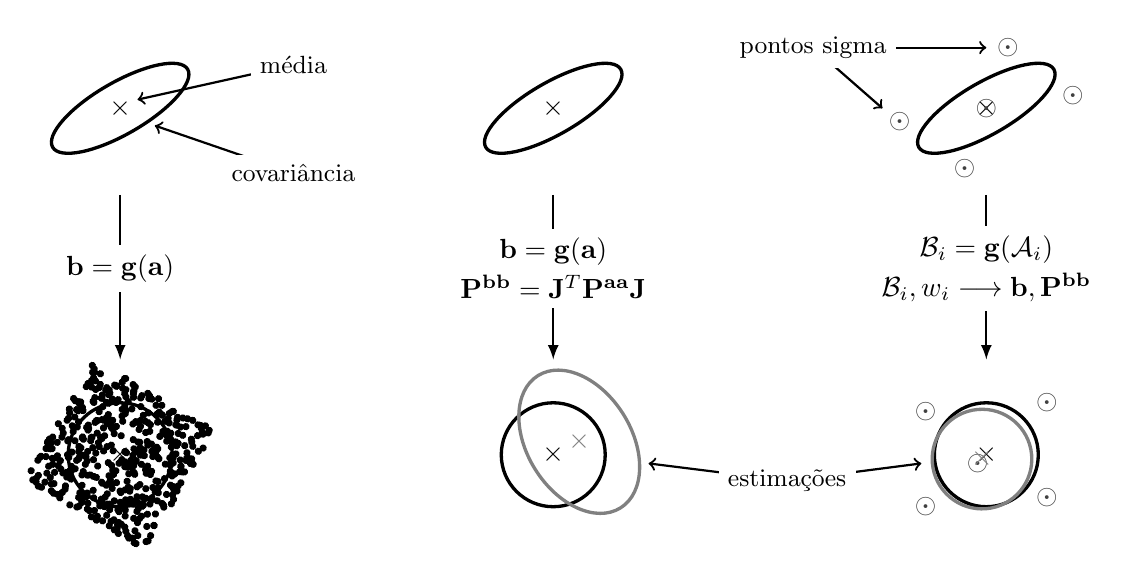
\begin{tikzpicture}[scale=1.1]
    \begin{scope}[rotate=-60]
        \draw plot[mark=*, only marks, mark size=1] file {data/unscented-cloudx.dat};
    \end{scope}

    \pgfmathsetseed{64698676}
    \draw plot[mark=*, only marks, mark size=1, samples=500, rotate around={60:(0, -4)}] ({0.8*rand}, {-4 + 0.8*rand});

    \foreach \i in {0,5,10} {
        \node[black] at (\i, 0) {$\bm{\times}$};
        \draw[very thick, black, rotate around={-60:(\i, 0)}] (\i, 0) ellipse (0.3 and 0.9);
        \node[black] at (\i, -4) {$\bm{\times}$};
        \draw[very thick, black] (\i, -4) circle (0.6);
    }

    \draw[-latex, thick] (0, -1) -- (0, -2.9);
    \node[fill=white] at (0, -1.85) {$\mathbf{b} = \mathbf{g}(\mathbf{a})$};

    % Linearized
    \draw[very thick, gray, rotate around={32:((5.3, -3.85))}] (5.3, -3.85) ellipse (0.6 and 0.9);
    \node[gray] at (5.3, -3.85) {$\bm{\times}$};

    \draw[-latex, thick] (5, -1) -- (5, -2.9);
    \node[fill=white, align=center] at (5, -1.85) {$\Bar{\mathbf{b}} = \mathbf{g}(\Bar{\mathbf{a}})$\\[2.5pt]$\mathbf{P}^{\mathbf{b}\mathbf{b}} = \mathbf{J}^T \mathbf{P}^{\mathbf{a}\mathbf{a}} \mathbf{J}$};

    % UT
    \draw[very thick, gray, rotate around={5:((9.95, -4.05))}] (9.95, -4.05) circle (0.575);
    \node[darkgray] at (10, 0) {$\bm{\odot}$};
    \node[darkgray] at (9.9, -4.1) {$\bm{\odot}$};
    \foreach \i in {-1, 1} {
        \node[darkgray] at (10 + 1*\i, 0.15*\i) {$\bm{\odot}$};
        \node[darkgray] at (10 + 0.25*\i, 0.7*\i) {$\bm{\odot}$};
        \node[darkgray] at (10 - 0.7*\i, -4 + 0.5*\i) {$\bm{\odot}$};
        \node[darkgray] at (10 + 0.7*\i, -4 + 0.6*\i) {$\bm{\odot}$};
    }
    \node[gray] at (9.95, -4.05) {$\bm{\times}$};

    \draw[-latex, thick] (10, -1) -- (10, -2.9);
    \node[fill=white, align=center] at (10, -1.85) {$\bm{\mathcal{B}}_i = \mathbf{g}(\bm{\mathcal{A}}_i)$\\[2.5pt]$\bm{\mathcal{B}}_i, w_i \longrightarrow \Bar{\mathbf{b}}, \mathbf{P}^{\mathbf{b}\mathbf{b}}$};

    \draw[->, thick] (2, 0.5) -- (0.2, 0.1);
    \draw[->, thick] (2, -0.75) -- (0.4, -0.2);
    \node[fill=white, align=center] at (2, 0.5) {\small média};
    \node[fill=white, align=center] at (2, -0.75) {\small covariância};

    \draw[->, thick] (7.7, -4.3) -- (6.1, -4.1);
    \draw[->, thick] (7.7, -4.3) -- (9.25, -4.1);
    \node[fill=white, align=center] at (7.7, -4.3) {\small estimações};

    \draw[->, thick] (8, 0.7) -- (10, 0.7);
    \draw[->, thick] (8, 0.7) -- (8.8, 0);
    \node[fill=white, align=center] at (8, 0.7) {\small pontos sigma};
\end{tikzpicture}

    \caption[Ilustração dos métodos de estimação de momentos]{Três modos de estimar os momentos da variável aleatória $\mathbf{b}$. À esquerda, (muitas) amostras do experimento são usadas para calcular as estatísticas reais da variável. Ao centro, os momentos são aproximados pelo modelo linearizado da função ($\mathbf{J}$ é o jacobiano de $\mathbf{g}$); erros na aproximação acabam sendo propagados para a estimação. À direita, temos a transformação \textit{unscented}, na qual um conjunto estratégico de pontos é utilizado para computar as estatísticas. Ilustração baseada em um desenho similar presente em~\cite{wan-2000}.}
    \label{fig:unscented:ut}
\end{figure}

\section{Filtro de Kalman \textit{Unscented}}

Com o problema bem definido e a transformação \textit{unscented} apresentada, derivar o filtro se torna relativamente simples. Tudo que é preciso fazer é encontrar as equações associadas às previsões $\hat{\mathbf{x}}_{n+1|n}$, $\mathbf{P}_{n+1|n}^{\mathbf{x}\mathbf{x}}$, $\hat{\mathbf{z}}_{n+1|n}$, $\mathbf{P}_{n+1|n}^{\bm{\nu}\bm{\nu}}$, e $\mathbf{P}_{n+1|n}^{\mathbf{x}\mathbf{z}}$, para que seja possível realizar as etapas de predição e correção alternadamente.

Precisamos primeiramente definir um novo vetor de estados, no qual se inclua $\mathbf{v}_n$. Deste modo, as estatísticas do ruído ``interno'' --- modelado como não-aditivo --- serão consideradas na estimação da média e da covariância do sistema. Assim, supondo que $\mathbf{v}_n \in \mathbb{R}^q$, o vetor de estados aumentado $\mathbf{x}^a_{n} \in \mathbb{R}^{(k + q)}$ é definido como
\begin{equation}
    \mathbf{x}^a_{n} = \begin{bmatrix}
        \mathbf{x}_n \\
        \mathbf{v}_n
    \end{bmatrix}.
    \symbl{$\mathbf{x}^a_{n}$}{Vetor de estados aumentado modelado pelo Filtro de Kalman \textit{Unscented}}
\end{equation}
Consequentemente, temos que a dinâmica do sistema agora é descrita por
\begin{equation}
    \mathbf{x}^a_{n+1} = \mathbf{f}(\mathbf{x}^a_{n}, \mathbf{u}_n),
\end{equation}
e a média e a covariância a serem usadas pela transformação \textit{unscented} serão
\begin{equation}
    \hat{\mathbf{x}}^a_{n|n} = \begin{bmatrix}
        \mathbf{x}_{n|n} \\
        \mathbf{0}
    \end{bmatrix},\ 
    \mathbf{P}^{\mathbf{x}^a\mathbf{x}^a}_{n|n} = \begin{bmatrix}
        \mathbf{P}^{\mathbf{x}\mathbf{x}}_{n|n} & \mathbf{P}^{\mathbf{x}\mathbf{v}}_{n|n} \\
        \mathbf{P}^{\mathbf{x}\mathbf{v}}_{n|n} & \mathbf{Q}_n
    \end{bmatrix}.
    \label{eq:unscented:augmented}
\end{equation}

Munidos de todas as definições necessárias, podemos agora descrever o algoritmo do Filtro de Kalman \textit{Unscented}. O passo de inicialização consiste em calcular as condições iniciais dos estados originais com
\begin{align}
    \hat{\mathbf{x}}_{0|0} &= E\{ \mathbf{x}_0 \},\\
    \mathbf{P}_{0|0}^{\mathbf{x}\mathbf{x}} &= E\{ (\mathbf{x}_0 - \hat{\mathbf{x}}_{0|0}) (\mathbf{x}_0 - \hat{\mathbf{x}}_{0|0})^T \},
\end{align}
para que o sistema aumentado comece com as condições $\hat{\mathbf{x}}^a_{0|0}$ e $\mathbf{P}^{\mathbf{x}^a\mathbf{x}^a}_{0|0}$ como descritas pela Equação~\eqref{eq:unscented:augmented}. Então, para $n \in \mathbb{N}$ variando de $0$ a infinito (ou até a última amostra de interesse), iteramos pelos seguintes passos:

\begin{enumerate}
    \item Em posse de $\hat{\mathbf{x}}^a_{n|n}$, estima-se a observação $\hat{\mathbf{z}}_{n|n}$, que é a saída do filtro.

    \item Com as Equações~\eqref{eq:unscented:sigma-first} a~\eqref{eq:unscented:sigma-last}, são calculados os $2(k + q) + 1$ pontos sigma associados a $\hat{\mathbf{x}}^a_{n|n}$, gerando assim o conjunto $\{\bm{\mathcal{X}}_{n|n,i}^a\}$.
    
    \item Os pontos sigma são mapeados pela função não-linear que descreve a dinâmica dos estados do sistema, ou seja,
    \symbl{$\bm{\mathcal{X}}_{\cdot,i}$}{Ponto sigma $i$ da entrada}
    \begin{equation}
        \bm{\mathcal{X}}_{n+1|n,i}^a = \mathbf{f}(\bm{\mathcal{X}}_{n|n,i}^a, \mathbf{u}_n).
    \end{equation}
    
    \item Com os coeficientes $w_i$ definidos na Equação~\eqref{eq:unscented:weights}, o novo vetor de estados e sua matriz de covariância são estimados como sendo
    \begin{gather}
        \hat{\mathbf{x}}_{n+1|n}^a = \sum_{i=0}^{2(k+q)} w_i \bm{\mathcal{X}}_{n+1|n,i}^a, \\
        \mathbf{P}^{\mathbf{x}^a\mathbf{x}^a}_{n+1|n} = \sum_{i=0}^{2(k+q)} w_i (\bm{\mathcal{X}}_{n+1|n,i}^a - \hat{\mathbf{x}}_{n+1|n}^a) (\bm{\mathcal{X}}_{n+1|n,i}^a - \hat{\mathbf{x}}_{n+1|n}^a)^T.
    \end{gather}

    \item Os pontos sigma são novamente mapeados, agora pela função que descreve a dinâmica de saída do sistema:
    \begin{equation}
        \symbl{$\bm{\mathcal{Z}}_{\cdot,i}$}{Ponto sigma $i$ da observação}
        \bm{\mathcal{Z}}_{n+1|n,i} = \mathbf{h}(\bm{\mathcal{X}}_{n+1|n,i}^a, \mathbf{u}_{n+1}).
    \end{equation}

    \item Com os pontos mapeados, estimam-se a próxima observação e sua covariância (lembrando-se de que o ruído $\mathbf{w}_n$ é pressuposto aditivo e independente),
    \begin{gather}
        \hat{\mathbf{z}}_{n+1|n} = \sum_{i=0}^{2(k+q)} w_i \bm{\mathcal{Z}}_{n+1|n,i}, \\
        \mathbf{P}^{\bm{\nu}\bm{\nu}}_{n+1|n} = \mathbf{R}_n + \sum_{i=0}^{2(k+q)} w_i (\bm{\mathcal{Z}}_{n+1|n,i} - \hat{\mathbf{z}}_{n+1|n}) (\bm{\mathcal{Z}}_{n+1|n,i} - \hat{\mathbf{z}}_{n+1|n})^T.
    \end{gather}

    \item Por fim, calculamos a matriz de covariância cruzada entre $\mathbf{x}_n^a$ e $\mathbf{z}$,
    \begin{equation}
        \mathbf{P}^{\mathbf{x}^a\mathbf{z}}_{n+1|n} = \sum_{i=0}^{2(k+q)} w_i (\bm{\mathcal{X}}_{n+1|n,i}^a - \hat{\mathbf{x}}_{n+1|n}^a) (\bm{\mathcal{Z}}_{n+1|n,i} - \hat{\mathbf{z}}_{n+1|n})^T.
    \end{equation}        

    \item A observação $\mathbf{z}_{n+1}$ é usada, em conjunto com as Equações~\eqref{eq:unscented:diff} a \eqref{eq:unscented:kalman-last} e as matrizes calculadas nas etapas anteriores, na correção das estimações do vetor de estados e sua matriz de covariância, gerando assim $\hat{\mathbf{x}}_{n+1|n+1}^a$ e $\mathbf{P}^{\mathbf{x}^a\mathbf{x}^a}_{n+1|n+1}$.
\end{enumerate}

Esse algoritmo é específico para o modelo descrito na Seção~\ref{section:unscented:formulation}, mas pode ser facilmente adaptado a outras hipóteses. Para considerar um ruído de observação não-aditivo, por exemplo, poderíamos definir uma versão aumentada do vetor de observação, a qual incluiria o vetor de ruído.

\section{Método proposto}
\label{section:unscented:model}

Durante toda a análise do filtro, pressupusemos que as funções não-lineares $\mathbf{f}$ e $\mathbf{h}$ eram previamente conhecidas. Afinal, o algoritmo é utilizado para estimar a memória do sistema, não sua dinâmica. Porém, em um problema de identificação, como o do trabalho, essa é justamente a incógnita que se quer descobrir. Assim, precisamos adaptar a estratégia para esse ângulo.

Quando nada se sabe sobre o comportamento interno do sistema, o que podemos fazer é definir funções --- idealmente genéricas, capazes de aproximar outros mapeamentos --- que dependam dos estados e de um conjunto de parâmetros. Então, dois filtros são executados de forma simultânea: um para a estimação dos estados, e outro para a estimação dos parâmetros. Este método é chamado de \emph{Filtro de Kalman Unscented Duplo}~\cite{wan-2000}. O primeiro subsistema é muito similar ao apresentado na Seção~\ref{section:unscented:formulation}, porém com uma entrada adicional, que é vetor de parâmetros $\bm{\omega}_n$\symbl{$\bm{\omega}_n$}{Vetor com os coeficientes do polinômio de Volterra usado no Filtro de Kalman \textit{Unscented}}:
\begin{align}
    \mathbf{x}_{n+1} &= \mathbf{f}(\mathbf{x}_n, \mathbf{u}_n, \bm{\omega}_n, \mathbf{v}_n), \\
    \mathbf{z}_n &= \mathbf{h}(\mathbf{x}_n, \bm{\omega}_n, \mathbf{u}_n) + \mathbf{w}_n.
\end{align}
Já o subsistema associado aos parâmetros é descrito por
\begin{align}
    \bm{\omega}_{n+1} &= \bm{\omega}_n + \mathbf{v}_n, \\
    \mathbf{z}_n &= \mathbf{h}(\mathbf{x}_n, \bm{\omega}_n, \mathbf{u}_n) + \mathbf{w}_n.
\end{align}
Embora pareça que a dinâmica desse subsistema acarrete na convergência dos coeficientes, o ruído de processo e o algoritmo de correção contribuem com uma ``inovação'' a cada nova amostra, resultando assim num filtro adaptativo.

Vamos agora finalmente associar a teoria apresentada aos elementos específicos do projeto. Para a função $h$ (escalar, já que a saída é unidimensional), optamos por usar um polinômio de Volterra~\cite{ogunfunmi-2007} de $P$-ésima ordem\symbl{$P$}{Ordem do polinômio de Volterra} que utilize as últimas $L$ amostras da entrada $x[n]$, ou seja,
\begin{equation}
    \symbl{$h(\dots)$}{Polinômio de Volterra do Filtro de Kalman \textit{Unscented}}
    h(\mathbf{x}_n, \bm{\omega}_n, \mathbf{u}_n) = \sum_{m=0}^{L-1} \omega_m x[n-m] + \sum_{m=0}^{L-1} \sum_{p=m}^{L-1} \omega_{m,p} x[n-m] x[n-p] + \dots.
\end{equation}
Dois fatores justificam essa escolha: em primeiro lugar, polinômios são capazes de aproximar (localmente) diversos mapeamentos complexos, portanto são funções genéricas o suficiente para serem usadas na modelagem de um sistema desconhecido. Além disso, os termos cruzados fazem com que a ``correlação instantânea'' entre amostras seja considerada na estimação, o que pode contribuir na reprodução de processamentos não-lineares com memória. Porém, ressaltamos o que foi dito no Capítulo~\ref{chapter:intro}: os coeficientes desse modelo crescem exponencialmente com a ordem do polinômio, portanto, devemos tomar cuidado na escolha de $L$ e $P$.

Com a dinâmica da saída definida, precisamos então caracterizar cada um dos vetores do sistema. A entrada será simplesmente o sinal não-distorcido,
\begin{equation}
    \mathbf{u}_n = x[n].
\end{equation}

O vetor $\bm{\omega}_n$ será composto por todos os parâmetros do polinômio,
\begin{equation}
    \symbl{$\omega_{i,\dots,j}$}{Coeficiente do polinômio de Volterra usado no Filtro de Kalman \textit{Unscented}}
    \bm{\omega}_n = \begin{bmatrix}
        \omega_0 & \cdots & \omega_{L-1} & \omega_{0,0} & \cdots & \omega_{L-1,\dots,L-1}
    \end{bmatrix}^T.
\end{equation}

Para que as amostras passadas possam ser utilizadas pela função, elas precisam ser armazenadas na memória do sistema. Assim, o vetor de estados será composto pelas $L-1$ amostras anteriores da entrada,
\begin{equation}
    \mathbf{x}_n = \begin{bmatrix}
        x[n-1] & x[n-2] & \cdots & x[n-L+1]
    \end{bmatrix}^T.
\end{equation}
Desse modo, a dinâmica interna do primeiro subsistema, descrita pela função $\mathbf{f}$, consiste apenas na inclusão de $x[n]$ como novo primeiro elemento do vetor de estados, e no deslocamento das demais amostras --- resultando no descarte de $x[n-L]$. O ruído de processo $\mathbf{v}_n$ é considerado aditivo em ambos os subsistemas.

Por fim, pode-se afirmar então que a o sinal desejado é descrito por
\begin{equation}
    d[n] = h(\mathbf{x}_n, \bm{\omega}_n, \mathbf{u}_n),
\end{equation}
porém temos apenas a observação ruidosa desse sinal, $\mathbf{z}_n = y[n] = d[n] + w_n$.

\section{Experimentos}

Em nossa última leva de experimentos, foram novamente utilizadas as duas faixas de áudio apresentadas na Seção~\ref{section:wf:experiments}: como sinal original, uma breve gravação da flauta hulusi (espectrograma na Figura~\ref{fig:wf:spectogram-reference}); como ruído, um diálogo de uma leitura dramática de \textit{Mansfield Park} (espectrograma na Figura~\ref{fig:wf:spectogram-dialogue}). Ambas as gravações permaneceram com os pré-condicionamentos anteriormente especificados (mono, taxa de amostragem de $44.1$~kHz, \textit{bitdepth} de 16~bits, ganho de normalização para 0~dB).

Desde a versão R2016b, o MATLAB conta com uma função nativa que implementa o Filtro de Kalman \textit{Unscented}, \texttt{unscentedKalmanFilter()}. Assim, o algoritmo foi elaborado instanciando dois filtros, um associado ao subsistema dos estados e outro associado ao subsistema dos coeficientes. Quase todos os valores padrão da função foram mantidos; apenas a variância do ruído de processo ($\sigma_{\mathbf{v}}^2 = 0.01$\symbl{$\sigma_{\mathbf{v}}^2$}{Variância do ruído de processo} para todos os experimentos) e a variância do ruído de saída (definidas individualmente) foram modificadas. Os filtros foram inicializados com vetores nulos. Por fim, foram estipulados $P=3$ e $L=3$ para o polinômio de Volterra; assim como no Filtro de Correntropia, valores maiores aumentavam de modo considerável o custo computacional do método, e resultavam em estimações apenas marginalmente melhores.

\subsection{\textit{Fades}}

Para testar a capacidade do algoritmo em identificar um sistema variante no tempo, foram aplicados à gravação original um \textit{fade-out} (com parâmetros $A_\text{i} = 1$ e $A_\text{f} = 0.2$) e um \textit{fade-in} (com parâmetros $A_\text{i} = 0.2$ e $A_\text{f} = 1$) em seu início e seu fim, respectivamente; cada efeito seguiu uma curva exponencial e durou cerca de 1.5 segundo. Nenhum ruído foi introduzido, porém a variância do ruído de saída foi considerada ser $\sigma_w^2 = 10^{-4}$\symbl{$\sigma_{\mathbf{w}}^2$}{Variância do ruído de saída}. Os resultados encontram-se na Tabela~\ref{tab:unscented:experiment-1}.
{\def\arraystretch{1.25}\tabcolsep=10pt
\begin{table}[!ht]
    \centering
    \caption[Resultados do primeiro experimento: \textit{fades}]{Resultados do primeiro experimento.}
    \label{tab:unscented:experiment-1}
    \begin{tabular}{cccc}
        \toprule
                         & SDR        & PAQM (MOS)   & $\log_{10}(R_{\text{nonlin}})$ \\
        \midrule
        $(d, x)$       & $-11.57$ dB & $1.17$  &  $-0.005$               \\
        $(d, \hat{d})$ & $98.25$ dB & $4.62$  &   $-0.004$              \\ \bottomrule
    \end{tabular}
\end{table}
}

O filtro não só foi capaz de acompanhar o processamento, como superou os resultados de ambos os métodos discutidos anteriormente. A provável justificativa para a qualidade da estimativa é o fato de que os coeficientes do polinômio são corrigidos de amostra em amostra --- não de janela em janela, como nas estratégias propostas para os outros dois filtros ---, dando assim mais dinamismo à estimação.

\subsection{\textit{Fades} com ruído aditivo}

Neste experimento, o diálogo foi somado à gravação gerada na subseção anterior, fazendo assim com que o sinal desejado se comportasse como trilha de fundo da mixagem. A SNR resultante foi de $-9.17$~dB. A variância do ruído de saída ótima para esse experimento (estipulada após diversos testes com diferentes valores) foi de $\sigma_w^2 = 4 \times 10^{4}$. Os resultados encontram-se na Tabela~\ref{tab:unscented:experiment-2}.
{\def\arraystretch{1.25}\tabcolsep=10pt
\begin{table}[!ht]
    \centering
    \caption[Resultados do segundo experimento: \textit{fades} com ruído aditivo]{Resultados do segundo experimento.}
    \label{tab:unscented:experiment-2}
    \begin{tabular}{cccc}
        \toprule
                         & SDR        & PAQM (MOS)   & $\log_{10}(R_{\text{nonlin}})$ \\
        \midrule
        $(d, x)$       & $-11.57$ dB & $1.17$  &  $-0.005$               \\
        $(d, \hat{d})$ & $16.56$ dB & $1.18$  &   $-0.027$              \\ \bottomrule
    \end{tabular}
\end{table}
}

No Capítulo~\ref{chapter:wiener}, vimos que a estimação gerada pelo Filtro de Wiener apresentou artefatos ``metálicos'' e ininteligíveis. Em contrapartida, ao se ouvir o sinal computado pelo Filtro de Kalman \textit{Unscented}, nota-se que o ruído ficou abafado, com baixa potência, mas ainda assim compreensível (ou seja, foi possível identificar as falas dos personagens).

\subsection{\textit{Soft clipping}}

Para avaliarmos a capacidade do filtro em estimar um processamento não-linear, aplicou-se o efeito de \textit{soft clipping} à gravação da flauta. O pico de amplitude foi limitado a $-7.5$~dB. A variância do ruído de saída foi novamente $\sigma_w^2 = 10^{-4}$. Os resultados encontram-se na Tabela~\ref{tab:unscented:experiment-3}.
{\def\arraystretch{1.25}\tabcolsep=10pt
\begin{table}[!ht]
    \centering
    \caption[Resultados do terceiro experimento: \textit{soft clipping}]{Resultados do terceiro experimento.}
    \label{tab:unscented:experiment-3}
    \begin{tabular}{cccc}
        \toprule
                         & SDR        & PAQM (MOS)   & $\log_{10}(R_{\text{nonlin}})$ \\
        \midrule
        $(d, x)$       & $19.56$ dB & $1.21$  &  $-0.016$               \\
        $(d, \hat{d})$ & $99.04$ dB & $4.62$  &   $-0.003$              \\ \bottomrule
    \end{tabular}
\end{table}
}

Não há muito o que comentar em relação aos resultados, além de que o filtro reproduziu satisfatoriamente o processamento aplicado. Não foi possível identificar nenhum artefato presente na estimação como ocorreu com os outros dois métodos.

\subsection{\textit{Soft clipping} com ruído aditivo}

Neste experimento, queremos novamente que o filtro estime o efeito de \textit{soft clipping}, porém agora com ruído aditivo adicionado à mixagem. A SDR da observação foi de $3.97$~dB. Para esse teste, a variância de ruído ótima (dentre os valores testados) foi de $\sigma_w^2 = 10^{4}$. Os resultados encontram-se na Tabela~\ref{tab:unscented:experiment-4}.
{\def\arraystretch{1.25}\tabcolsep=10pt
\begin{table}[!ht]
    \centering
    \caption[Resultados do quarto experimento: \textit{soft clipping} com ruído aditivo]{Resultados do quarto experimento.}
    \label{tab:unscented:experiment-4}
    \begin{tabular}{cccc}
        \toprule
                         & SDR        & PAQM (MOS)   & $\log_{10}(R_{\text{nonlin}})$ \\
        \midrule
        $(d, x)$       & $19.56$ dB & $1.21$  &  $-0.016$               \\
        $(d, \hat{d})$ & $27.27$ dB & $1.18$  &   $-0.016$              \\ \bottomrule
    \end{tabular}
\end{table}
}

Houve uma melhoria no valor da SDR, e, curiosamente, uma queda na PAQM. Ao se ouvir a estimação resultante, observa-se um comportamento similar ao do segundo experimento: o filtro conseguiu reproduzir o efeito aplicado ao sinal original, mas não removeu por completo a faixa de diálogo, que ficou agressivamente abafada.

\subsection{\textit{Fades} e codificação com perdas}

Nosso objetivo agora é avaliar a capacidade do método de reproduzir não só um processamento linear, como também um não-linear aplicado em seguida. Para isso, a gravação gerada no primeiro experimento foi comprimida com uma codificação MP3 com taxa de bits constante de 56~kbps. Assim como nos outros testes em que o diálogo não foi adicionado, a variância do ruído de saída foi estipulada como sendo $\sigma_w^2 = 10^{-4}$. Os resultados encontram-se na Tabela~\ref{tab:unscented:experiment-5}.
{\def\arraystretch{1.25}\tabcolsep=10pt
\begin{table}[!ht]
    \centering
    \caption[Resultados do quinto experimento: \textit{fades} e codificação com perdas]{Resultados do quinto experimento.}
    \label{tab:unscented:experiment-5}
    \begin{tabular}{cccc}
        \toprule
                         & SDR        & PAQM (MOS)   & $\log_{10}(R_{\text{nonlin}})$ \\
        \midrule
        $(d, x)$       & $-14.77$ dB & $1.17$  &  $-0.032$               \\
        $(d, \hat{d})$ & $66.78$ dB & $4.50$  &   $-0.004$              \\ \bottomrule
    \end{tabular}
\end{table}
}

De todos os experimentos executados neste projeto, este talvez seja o mais surpreendente. O processamento aplicado por um algoritmo de compressão com perdas é altamente complexo; assim, é no mínimo admirável o nível de fidelidade da estimação do filtro, embora parte desses resultados seja consequência da emulação da distorção linear.

\subsection{\textit{Fades} com ruído aditivo e codificação com perdas}

Neste último experimento, queremos verificar se o filtro ainda é capaz de reproduzir o efeito da codificação com perdas quando ruído aditivo é introduzido antes do processamento. Para gerar o sinal observado, aplicou-se a codificação MP3 de 56~kbps na mixagem do segundo experimento. Após testarmos diferentes valores, a variância do ruído da saída foi estipulada como sendo $\sigma_w^2 = 2 \times 10^{3}$. Não foi possível calcular a SNR dessa observação, mas podemos estimar seu limite superior como sendo $-9.17$~dB. Os resultados encontram-se na Tabela~\ref{tab:unscented:experiment-6}.
{\def\arraystretch{1.25}\tabcolsep=10pt
\begin{table}[!ht]
    \centering
    \caption[Resultados do sexto experimento: \textit{fades} com ruído aditivo e codificação com perdas]{Resultados do sexto experimento.}
    \label{tab:unscented:experiment-6}
    \begin{tabular}{cccc}
        \toprule
                         & SDR        & PAQM (MOS)   & $\log_{10}(R_{\text{nonlin}})$ \\
        \midrule
        $(d, x)$       & $-14.77$ dB & $1.17$  &  $-0.032$               \\
        $(d, \hat{d})$ & $5.85$ dB & $1.17$  &   $-0.148$              \\ \bottomrule
    \end{tabular}
\end{table}
}

Como podemos ver, a única medida que apresentou melhoria foi a SDR. Ao ouvirmos a gravação resultante, percebe-se que foi introduzido um ruído ``metálico'' constante pelo método; além disso, o diálogo se manteve presente (embora abafado, como nos outros casos), e foi possível ouvir a presença de distorções indesejadas ao sinal de interesse (muito similares ao efeito de \textit{clipping}).